\documentclass[11pt, a4paper]{article}
\usepackage[top=2cm, bottom=3cm, left=2.5cm, right=2.5cm]{geometry}
\usepackage{amsmath,amsthm,amsfonts,amssymb,amscd, fancyhdr, color, comment, graphicx, environ}
\usepackage{float}
\usepackage{mathrsfs}
%\usepackage{unicode-math}
\usepackage{lastpage}
\usepackage[dvipsnames]{xcolor}
\usepackage[framemethod=TikZ]{mdframed}
\usepackage{enumerate}
\usepackage[shortlabels]{enumitem}
\usepackage{fancyhdr}
\usepackage{indentfirst}
\usepackage{listings}
\usepackage{sectsty}
\usepackage{thmtools}
\usepackage{shadethm}
\usepackage{hyperref}
\usepackage{setspace}
\usepackage{biblatex}

\addbibresource{ref.bib}

\hypersetup{
    colorlinks=true,
    linkcolor=blue,
    filecolor=magenta,      
    urlcolor=blue,
}

%%%%%%%%%%%%%%%%%%%%%%%%%%%%%%%%%%%%%%%%%%%%%%%%%%%%%%%%%%%%%%%%%%
%%%%%%%%%%%%%%%%%%%%%%%%%%%%%%%%%%%%%%%%%%%%%%%%%%%%%%%%%%%%%%%%%%
%Environment setup

\mdfsetup{skipabove=\topskip,skipbelow=\topskip}
\newrobustcmd\ExampleText{
}

\mdtheorem[style=theoremstyle]{Problem}{Problem}
\newenvironment{Solution}{\textbf{Solution.}}

%%%%%%%%%%%%%%%%%%%%%%%%%%%%%%%%%%%%%%%%%%%%%%%%%%%%%%%%%%%%%%%%%%
%%%%%%%%%%%%%%%%%%%%%%%%%%%%%%%%%%%%%%%%%%%%%%%%%%%%%%%%%%%%%%%%%%
%Fill in the appropriate information below
\newcommand{\norm}[1]{\left\lVert#1\right\rVert}     
\newcommand\course{Course}                      % <-- course name   
\newcommand\hwnumber{1}                         % <-- homework number
\newcommand\Information{XXX/xxxxxxxx}           % <-- personal information
%%%%%%%%%%%%%%%%%%%%%%%%%%%%%%%%%%%%%%%%%%%%%%%%%%%%%%%%%%%%%%%%%%
%%%%%%%%%%%%%%%%%%%%%%%%%%%%%%%%%%%%%%%%%%%%%%%%%%%%%%%%%%%%%%%%%%
%Page setup
\pagestyle{fancy}
\headheight 35pt
\lhead{\today}
\rhead{
\includegraphics[width=3cm]{logo-mpu.png}} % <-- school logo(please upload the file first, then change the name here)
\lfoot{}
\pagenumbering{arabic}
\cfoot{\small\thepage}
\rfoot{}
\headsep 1.2em
\renewcommand{\baselinestretch}{1.25}       
\mdfdefinestyle{theoremstyle}{%
linecolor=black,linewidth=1pt,%
frametitlerule=true,%
frametitlebackgroundcolor=gray!20,
innertopmargin=\topskip,
}
%%%%%%%%%%%%%%%%%%%%%%%%%%%%%%%%%%%%%%%%%%%%%%%%%%%%%%%%%%%%%%%%%%
%%%%%%%%%%%%%%%%%%%%%%%%%%%%%%%%%%%%%%%%%%%%%%%%%%%%%%%%%%%%%%%%%%
%Add new commands here
\renewcommand{\labelenumi}{\alph{enumi}}
\newcommand{\Z}{\mathbb Z}
\newcommand{\R}{\mathbb R}
\newcommand{\Q}{\mathbb Q}
\newcommand{\NN}{\mathbb N}
\DeclareMathOperator{\Mod}{Mod} 
\renewcommand\lstlistingname{Algorithm}
\renewcommand\lstlistlistingname{Algorithms}
\def\lstlistingautorefname{Alg.}
%%%%%%%%%%%%%%%%%%%%%%%%%%%%%%%%%%%%%%%%%%%%%%%%%%%%%%%%%%%%%%%%%%
%%%%%%%%%%%%%%%%%%%%%%%%%%%%%%%%%%%%%%%%%%%%%%%%%%%%%%%%%%%%%%%%%%
%Begin now!

\begin{document}

\begin{titlepage}
    \begin{center}
        \vspace*{1.5cm}
            
        \Huge
        \textbf{The smart door lock and smart NFC card based on IOT}
            
        \vspace{3cm}    
        \huge
        
        
            
        \vspace{2cm}
        \Large
            
        \textbf{Group 5}                                         % <-- author

        \vspace{1.5cm}

        \textbf{P2213011 Ruizhe Zhou, Retro}                     % <-- author

        \textbf{P2212852 Yuan Duan, Hector}                      % <-- author

        \textbf{P2212871 Dashun Zheng, Dawson}                   % <-- author

        \textbf{P2212952 Di Kang, Vincent}                       % <-- author
        
        %P2212852 段渊 Yuan Duan, Hector
        %P2212871 鄭大順 Dashun Zheng, Dawson
        %P2212952 康笛 Di Kang, Vincent
        %P2213011 周瑞哲 Ruizhe Zhou, Retro
        
        \vfill
        
        
            
        \vspace{1cm}
            
        
\includegraphics[width=0.7\textwidth]{logo-mpu.png}
        \\
        
        \Large
        
        \textbf{\today}
            
    \end{center}
\end{titlepage}

\newpage

\vspace{1cm}

\begin{center}

\tableofcontents

\end{center}

\newpage

\section{Project Description}

\subsection{Background}

As the fast development and revolution in Internet, communication, texting and electron technology, the IC card is more and more applicated everywhere in people's daily lives, even become a necessity in daily traveling.
The significant growth in the number of smart card issuance, thus the "Single function" development policies of different smart card manufacturers, the IC card caused a brand-new problem which brings fast and convenience at the same time: Individuals need to carry more and more smart cards to meet the various needs of daily travel.

\subsection{Project Overview}
With the significant growth in the number of smart card issuance, the smart cards have caused new problems while bringing convenience and speed to people's daily lives, thus, we design a smart card with NFC technology, which could store multiple cards' information, and it has the specific function of NFC card, which have a electronic ink screen to display some information.

Therefore, cards that people carry with them will become a problem that people often worry about while traveling around. And the loss of cards will cause a bunch of trouble, such as the loss of money, the loss of identity, and the loss of property. Therefore, we design a smart card with NFC technology, which could store multiple cards' information, and it has the specific function of NFC card, which have a electronic ink screen to display some information.
The smart card is a combination of IC card and NFC card, which can be used as a IC card and NFC card, which can store multiple cards' information, and it has the specific function of NFC card, which have a electronic ink screen to display some information.

Simultaneously, we also design a door lock system, which can be used to open the door lock by sending AT commands to the module while the NFC card reader received the unlock signal from the Smart NFC card.
The system can also be used as a relay to control the power of the door lock.

\subsection{Project Architecture}

For the Smart E-ink NFC card, we integrated the NFC card simulater and a E-ink screen to show some information on it. The information on the E-ink screen can be updated by chip ST25DV, which can communicate with the phone with a Android app under NFC protocol.

The NFC card simulation is processed by the STM32L051 chip and data is stored in different UID chips. The STM32L051 can also communicate with the phone in another Android application to overwrite the NFC card data into the chip.

For the door lock module, we used GD32 chip with W5500 Ethernet chip as a network relay to perform power-off and power-on operations by accepting AT commands from the back-end.

For the backend development, we used Java and Kotlin language, the main stream Spring Boot framework and MySQL database as the basis for the development and running on the cloud platform.
For security, we use the Shiro security rights management framework, the JWT single sign-on module to verify the user's identity.
All the network requests and background function calls are stored in the Log4j2 database.

The IC card simulation is quite simple, which we integrate a few UID chip, and shared the same antenna, and we can switch cards by a dial wheel. At the good side, we can treat L-ink as a collection of multiple individual cards, copying and swiping are straightforward, but in another hand, as many cards are added, the number of buttons will increase.


\section{Underlying Principle}

\subsection{NFC Technology}
The Near Field Communication (NFC) technology is a short distance high frequency communication technology. NFC technology is developed from the integration of contactless radio frequency identification (RFID) and interconnection technology, which contactless readers, contactless cards and point-to-point functions are integrated into a single chip, allowing any two devices to be close together and communicate between devices without the need for plug-in cables.

\begin{center}
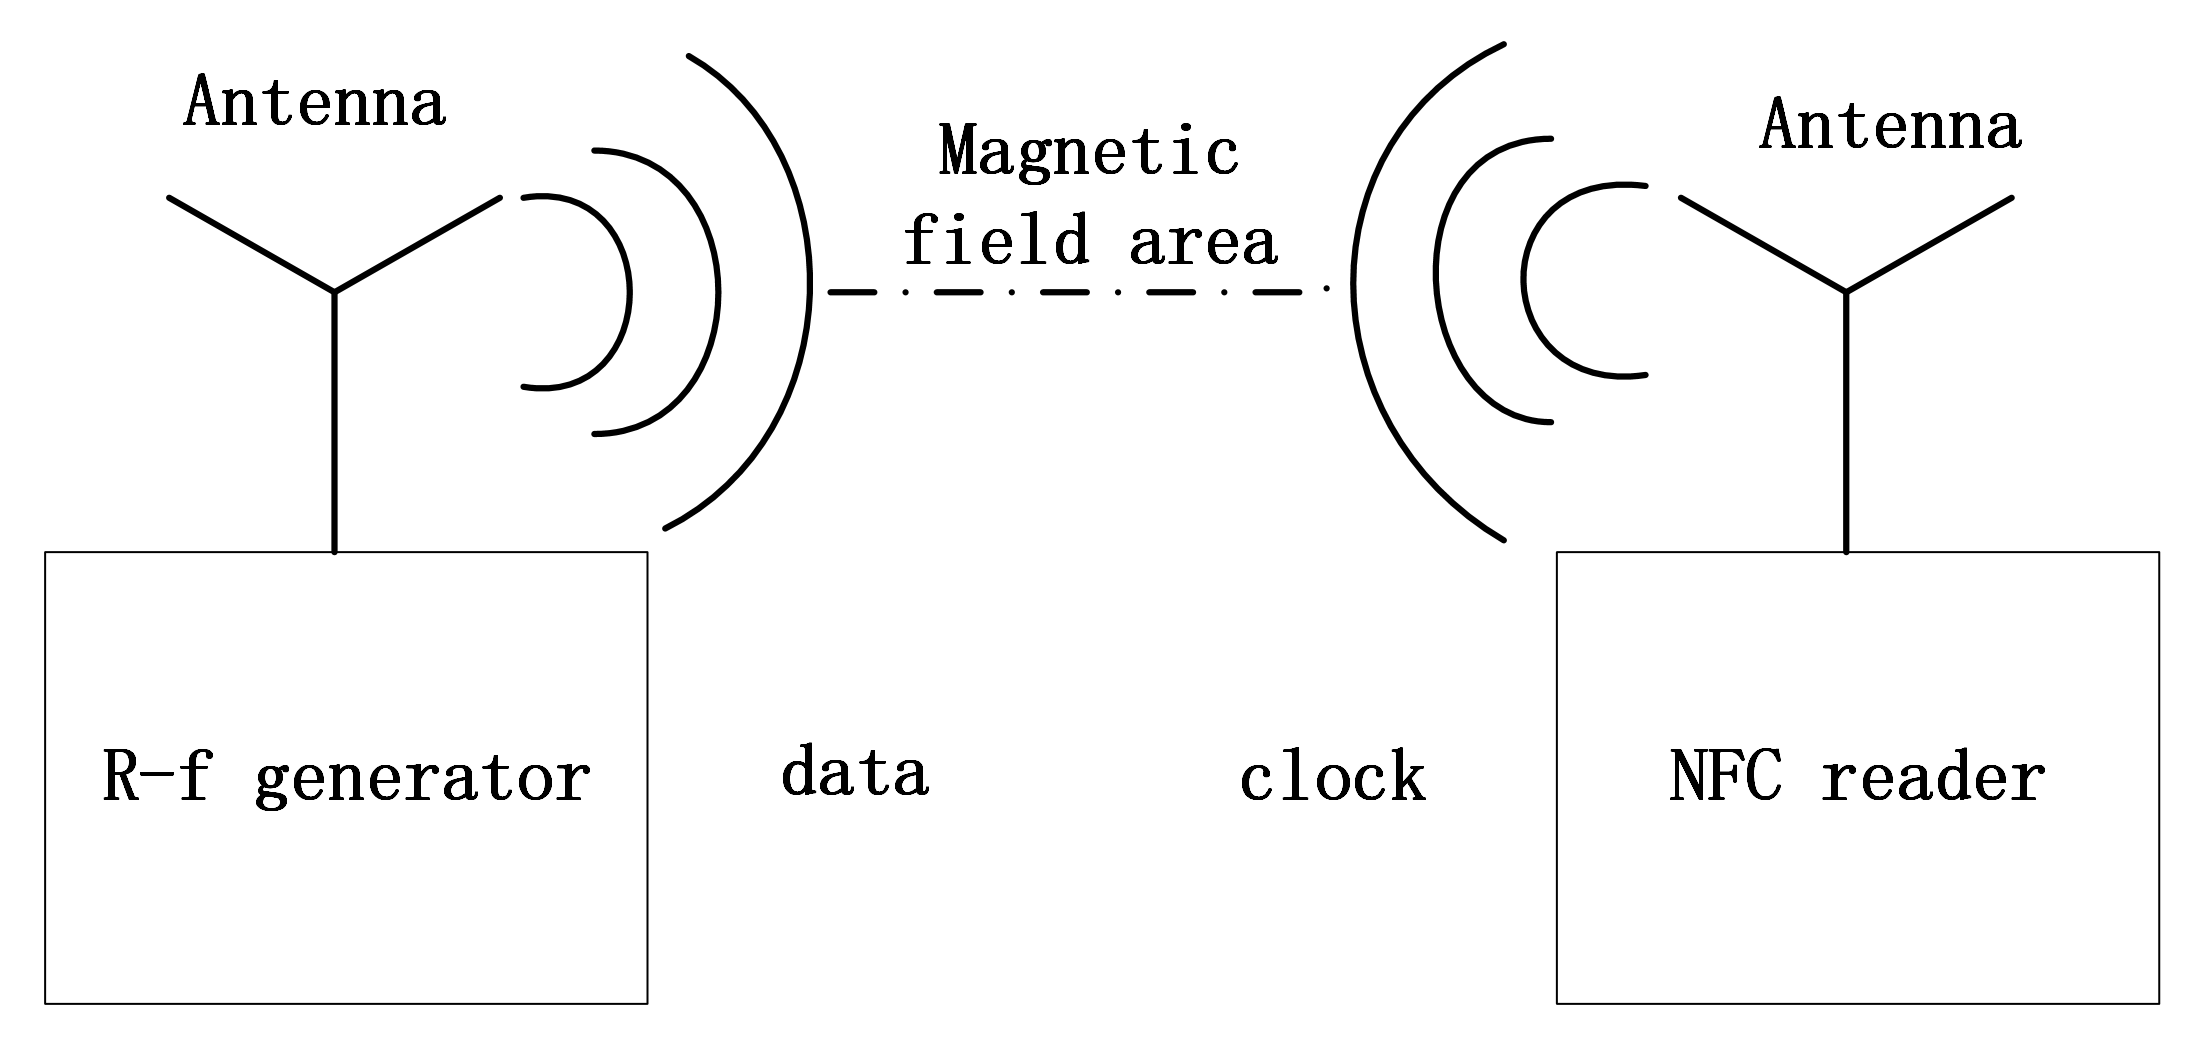
\includegraphics[scale=0.4]{pic1.png}
\\
Fig. 1: NFC working principle
\end{center}

NFC technology transmits information through inductive coupling. The working principle of NFC is shown in Figure 1. After the NFC-enabled device boots, continuously generates radio frequencies (RF) with a center frequency of 13.56MHz signal. If there is an NFC tag in the signal magnetic field fluctuation range, the tag will initiate the tag RF signal generation circuit with a current generated by electromagnetic induction, which will generates a feedback signal after the frequency property is changed, what will make the   reader detects the feedback signal of the tag to determine whether there is a tag around. The two NFC devices then establish a communication connection through magnetic field induced energy transfer and feedback signal acquisition and recognition, according to NFC protocol to enable identification and data exchange between close-range and NFC-compatible devices.

\subsection{AT Command and Socket Protocol}
AT Commands, developed by Dennis Hayes, are used to set data connections. The set of short string commands allows developers to set up calls with a modem, as well as perform far more complex tasks.

Socket is a software structure within a network node of a computer network that serves as an endpoint for sending and receiving data across the network.

In this project, the AT command is sent from the back-end to the relay using the Socket protocol, and the relay controls the door lock, as in Figure 2.
\begin{center}
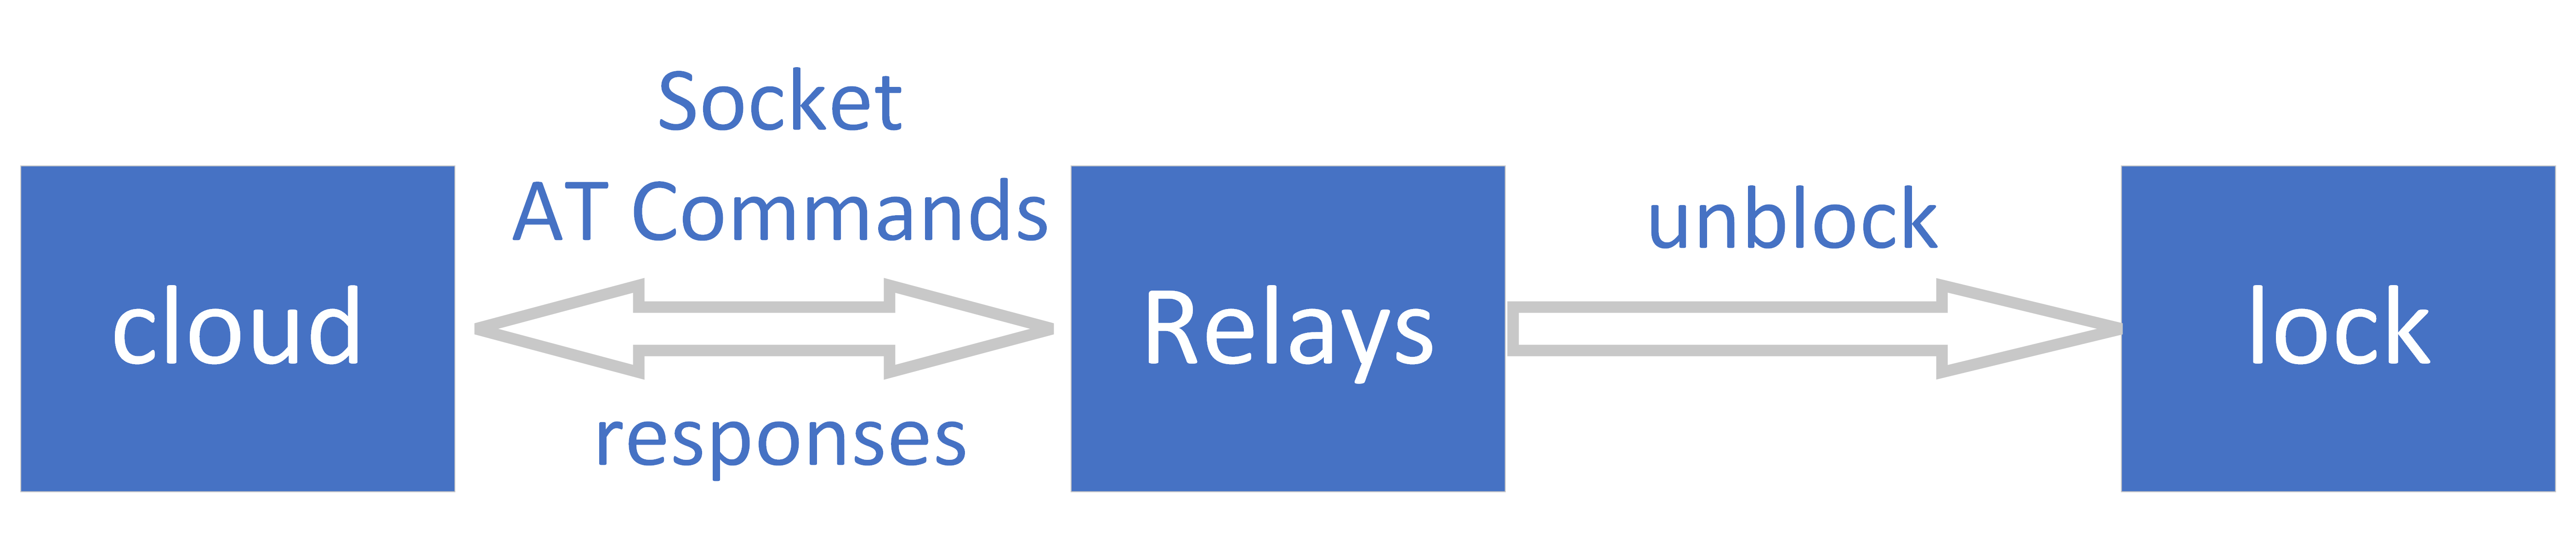
\includegraphics[scale=0.2]{pic2.png}
\\
Fig. 2: data flow diagram
\end{center}

\section{System Architecture}
To the design specification, we need to consider that the system involves the hardware part and the software part.
Thus, we need to obey the design specification as following:

\begin{enumerate}[1.]
    \item Provide a network interface, to make sure the system's scalability.
    \item Ensure the security of the system and the rubustness of the system, to make sure the system's reliability that could operate under any harsh conditions.
    \item Using more standard and open source components, to make sure the system's maintainability and the system functions' development.
\end{enumerate}


\subsection{Hardware Architecture}

The selection of the hardware components is mainly based on the following considerations:

\begin{enumerate}[1.]
    \item Provide a Internet controler chip, to send AT command by using the Socket protocol.
    \item At lease exist a switch signal module, to control the open and close of the door lock.
    \item Use an ARM based develop board as the network relay and have enough compute ability to handle the E-ink screen and massage handling.
    \item The selected chip needs to support NFC-related protocols.
\end{enumerate}

In conclution, we choose the GD32 chip as the network relay, and the W5500 chip as the Internet controller chip.
At the same time, for the smart E-ink NFC card, we choose the ST25DV chip as the NFC communication chip and the STM32L051 as the master control chip.

\subsubsection{Smart E-ink NFC Card}

For the Smart NFC Card, we mainly used 2$\times$IC chip, what are STM32L051 and ST25DV. The electronic ink screen is a $200 \times 200$ single color screen.

ST25DV communicate with STM32 chip through I2C bus as NFC's Physical Layer, which have 2 main functions, the energy harvesting and the NFC communication.
However, the ST25DV is only responsible for NFC communication with mobile phones, not for the read and write funtion for IC card, thus the ST25DV only supports ISO 15693's RFID protocol, but the IC card we commonly use is for ISO 14443 protocol, so we cannot directly use this chip to simulate IC card.


\subsubsection{Smart Door Lock System}

For the Smart Door Lock System, we integrated the NFC card reader, the magnetic door lock and a Internet controler to meet those needs.


\subsection{Software Architecture}
Using JAVA and Kotlin language as the basis for Spring Boot framework design and development of smart door lock system, through the single instance pattern to develop, using Spring Data persistence layer control MySQL database, and can be properly configured Web site, and can be well designed database and properly connected to the database.  The overall implementation of remote unlocking, access control management, user management, door opening records and other functions.  Consider its security, unauthorized third-party access, complete logs, etc.

\section{validation}
\subsection{Hardware Validation}

For the hardware validation, we mainly use the simulation software, oscilloscope, DC source and the multimeter to test the hardware make sure there exist no unexpected bug in our device.

For the simulation software, we choose the Proteus, which is a professional circuit simulation software.
The simulation software is used to simulate the hardware circuit, and it can simulate the hardware circuit and the software program.

For the oscilloscope, we use the Rigol DS1054Z, which is a 4-channel oscilloscope.
The oscilloscope is used to test the signal of the hardware circuit, and it can display the signal of the hardware circuit.

For the DC source, we use the DS2482, which is a 16-bit ADC.
The DC source is used to test the voltage of the hardware circuit, and it can display the voltage of the hardware circuit.

For the multimeter, we use the Rigol DM3058, which is a 5.5-digit multimeter.
The multimeter is used to test the resistance of the hardware circuit, and it can display the resistance of the hardware circuit.

According multiple tests mentioned above, all the hardware validations showed that the hardware circuit works well.
\subsection{Software Validation}
For the back-end functional validation, we mainly use Postman to send post requests. The back-end will return the validation result.Use Socket protocol to create TCP connection and send AT command to GD32 hardware.

Software validation environment we used JDK11, MySQL8.

After several verification, the software function works well.
\subsection{Summary}
According to the hardware validation and the black-box test, the system works well and no unexpected results or bugs have been found.

\section{Conclusion}
\subsection{Summary}
\subsection{Future Works}


\nocite{*}
\printbibliography


\end{document}
%%%%%%%%%%%%%%%%%%%%%%%%%%%%%%%%%%%%%%%%%%%%%%%%%%%%%%%%%%%%%%%%%%
%%%%%%%%%%%%%%%%%%%%%%%%%%%%%%%%%%%%%%%%%%%%%%%%%%%%%%%%%%%%%%%%%%